\subsection{Deployment Diagrams}
        \begin{center}
        \begin{figure}[!htp]
        \begin{center}
         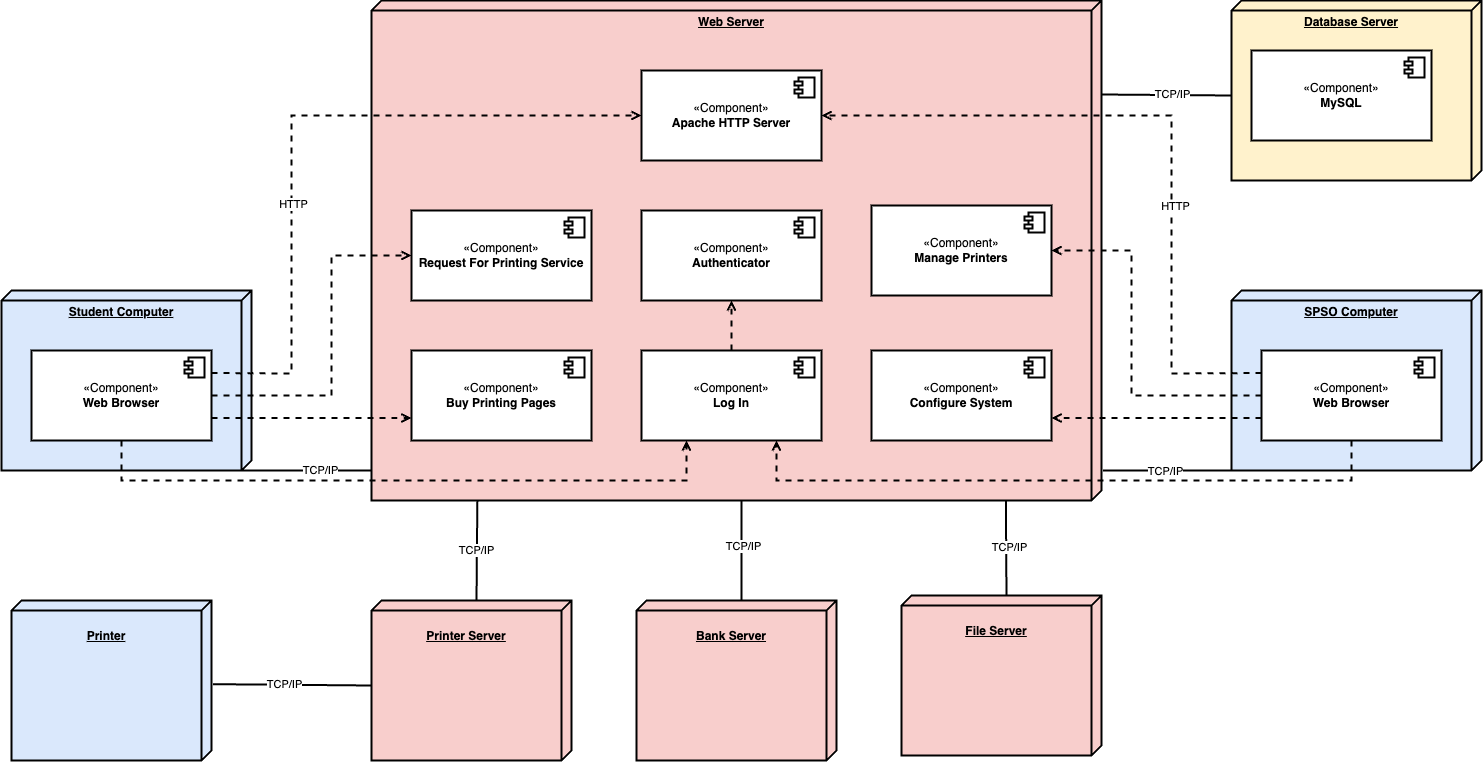
\includegraphics[scale=0.3]{images/Task3/Deployment Diagram/DeploymentDiagram(v1).drawio.png}
        \end{center}
        \end{figure}
        \end{center}

        \textbf{Mô tả:}
        \begin{itemize}
            \item Người dùng (sinh viên, người quản lí) sẽ  kết nối tới Web Server bằng Web Browser qua giao thức TCP/IP.
            \item Web Server sẽ cung cấp các dịch vụ và giao diện cho sinh viên và nhân viên quản lí:
            \begin{itemize}
                \item Dịch vụ sinh viên: Tính năng chính: đăng nhập (bao gồn Login, Change Password, Reset Password), tạo yêu cầu in (Request for printing service), mua thêm trang in (Buy Printing Pages) và thanh toán khi mua trang in (Online Payment). Ngoài ra còn có các tính năng phụ như: sinh viên có thể xem nhật kí sử dụng dịch vụ in của mình.
                \item Dịch vụ nhân viên quản lí: đăng nhập (Login, ChangePassword, Reset Password), quản lí các máy in (Manage Printers), cấu hình hệ thống (Configure System). Ngoài ra còn có một số tính năng phụ như: xem nhật kí sử dụng dịch vụ in của sinh viên, xem báo cáo thông kê về sử dụng dịch vụ in hằng tháng của hệ thống.
            \end{itemize}
            \item Web Server sẽ giao tiếp với Database Server qua qua giao thức TCP/IP.
            \item Database Server sử dụng mySQL và chứa các dữ liệu về sinh viên (student), nhân viên (SPSO), máy in (printer), tập tin (file), yêu cầu in (print request), thanh toán (payment), cấu hình hệ thống (configuration) v.v. Website sẽ tương tác với dữ liệu này thông qua REST API.
            \begin{itemize}
                \item REST sử dụng các yêu cầu HTTP như GET, PUT, POST và DELETE để quản lý các hoạt động CRUD (Create, Read, Update, and Delete).
                \item Dữ liệu được trả về với định dạng JSON.
            \end{itemize}
            
        \end{itemize}